
\documentclass[10pt]{article}
\usepackage[utf8]{inputenc}
\usepackage{kotex}
\usepackage{graphicx}
\usepackage{subfigure}
\usepackage{titling}
\setlength{\droptitle}{-2cm}
\usepackage{array}
\usepackage{amssymb}
\usepackage{amsmath}
\usepackage{siunitx} 
\usepackage{enumerate} 
\usepackage{pgfplots}
\usepackage{pgfplotstable}
\usepackage{tikz,pgfplots}
\usepackage{wasysym}
\usepackage{geometry}
\usepackage{authblk}
\usepackage{kotex}
\usepackage{bibunits}
\usepackage{tabularx}
\usepackage{hyperref}
\usepackage{pythonhighlight}

\geometry{
    a4paper,
    total={170mm,257mm},
    left=20mm,
    top=20mm,
}

\title{\textbf{Mathematical Foundation of DNN : HW 5}}
\author{Jeong Min Lee}

\begin{document}
\maketitle

\section{}
In this problem, I dervied the representation of each gradient, considering the result of problem6 at hw4.
Considering the forward pass in the first half of the code, the following relation is held, which does not agree to the notation in this problem.
\begin{equation*}
    y[l] = S(A_{list}[l-1]@y[l-1] + b_{list}[l-1])
\end{equation*}
Furthermore, due to the confusion from the notation, I introduced following definitions.
\begin{equation*}
    db_l = {d\over db_l}loss, \quad dy_l = {d\over dy_l}loss, \quad  dA_l = {d\over dA_l}loss
\end{equation*}
According to those notations, the code that calculate the each gradient can be implemented, easily.
\begin{align*}
    db_l &= {d\over db_l}loss \\
    &= {d\;loss\over dy_{l+1}} {d y_{l+1}\over db_l} \\
    &= dy_{l+1}{d \over db_l} S(A_ly_l + b_l)\\
    &= dy_{l+1}\text{diag}(S^\prime(A_ly_l + b_l))
\end{align*}

\begin{align*}
    dA_l &= {d\over dy_l}loss \\
    &= {d\; loss \over dy_L}{dy_L\over dA_l} \\
    &= dy_L \text{diag}(S^\prime(A_ly_l+b_l)) \left(\partial y_L\over \partial y_{l+1}\right)^T y_l^T \\
    &= \text{diag}S^\prime(A_ly_l+b_l)dy_{l+1}^Ty_l^T\quad \left(\because dy_l = {d\; loss \over dy_l} = {d \; loss \over dy_L}{d\; y_L\over dy_l} = dy_L{d y_L \over dy_l} \right) \\
    &= db_l^Ty_l^T
\end{align*}

\begin{align*}
    dy_l &= {d\over \; loss dy_{l+1}}{dy_{l+1}\over dy_l} \\
    &= dy_{l+1} {d\over dy_l} S(A_ly_l + b_l) \\
    &= dy_{l+1}S^\prime(A_ly_l+b_)A_l \\
    &= db_lA_list
\end{align*}


According to the results above, I implemented the python code as follow. 
As a result,the gradient calculation from the following code is identical to that of audograd. This implies that the code below is good implementation for backpropagation. 
\begin{python}
import torch
from torch import nn

def sigma(x):
    return torch.sigmoid(x)
def sigma_prime(x):
    return sigma(x)*(1-sigma(x))


torch.manual_seed(0)
L = 6
X_data = torch.rand(4, 1)
Y_data = torch.rand(1, 1)

A_list,b_list = [],[]
for _ in range(L-1):
    A_list.append(torch.rand(4, 4))
    b_list.append(torch.rand(4, 1))
A_list.append(torch.rand(1, 4))
b_list.append(torch.rand(1, 1))

# Option 3: implement backprop yourself
y_list = [X_data]
y = X_data
for ell in range(L):
    S = sigma if ell<L-1 else lambda x: x
    y = S(A_list[ell]@y+b_list[ell])
    y_list.append(y)


dA_list = []
db_list = []
dy = y-Y_data  # dloss/dy_L
for ell in reversed(range(L)):
    S = sigma_prime if ell<L-1 else lambda x: torch.ones(x.shape)
    A, b, y = A_list[ell], b_list[ell], y_list[ell] # A = A_l, b = b_l, y_l

    db = torch.mm(dy,torch.diag(S(A@y + b).flatten()))   # dloss/db_ell
    dA = torch.mm(y, db).T   # dloss/dA_ell
    dy = torch.mm(db, A)     # dloss/dy_{ell-1}
    

    dA_list.insert(0, dA)
    db_list.insert(0, db)

print(dA_list[0])
print(db_list[0])
\end{python}
\begin{python}
tensor([[2.3943e-05, 3.7064e-05, 4.2687e-06, 6.3700e-06],
        [3.4104e-05, 5.2794e-05, 6.0804e-06, 9.0735e-06],
        [2.4438e-05, 3.7831e-05, 4.3571e-06, 6.5019e-06],
        [2.0187e-05, 3.1250e-05, 3.5991e-06, 5.3707e-06]])
tensor([4.8247e-05, 6.8722e-05, 4.9245e-05, 4.0678e-05])

tensor([[2.3943e-05, 3.7064e-05, 4.2687e-06, 6.3700e-06],
        [3.4104e-05, 5.2794e-05, 6.0804e-06, 9.0735e-06],
        [2.4438e-05, 3.7831e-05, 4.3571e-06, 6.5019e-06],
        [2.0187e-05, 3.1250e-05, 3.5991e-06, 5.3707e-06]])
tensor([[4.8247e-05, 6.8722e-05, 4.9245e-05, 4.0678e-05]])
\end{python}


\section*{2}
This problem can be solved by applying the chain rule, repeatedly.
\begin{align}
    {\partial y_L \over \partial b_i} &= {\partial y_L \over \partial y_{L-1}} {\partial y_{L-1}\over \partial y_{L-2}}\cdots {\partial y_{i+1}\over \partial y_{i}}{\partial y_i \over \partial b_i} \\
    &= \text{diag}(\tilde{y_L})A_L \text{diag}(\sigma^\prime(\tilde{y}_{L-1}))A_{L-1}\cdots\text{diag}(\sigma^\prime(\tilde{y}_{i+1}))A_{i+1}\text{diag}(\sigma^\prime(\tilde{y}_i))
\end{align} 
\begin{align}
    {\partial y_L \over \partial A_i} &= \text{diag}(\sigma^\prime(\tilde{y}_i))\left({\partial y_L \over \partial y_i}\right)^Ty_{i-1}^T
\end{align}
where ${\partial y_L \over \partial y_i} = {\partial y_L \over \partial y_{L-1}} {\partial y_{L-1} \over \partial y_{L-2}} \cdots {\partial y_{i+1} \over \partial y_i} = \text{diag}(\tilde{y}_L)A_L\text{diag}(\sigma^\prime(\tilde{y}_{L-1}))A_{L-1} \cdots \text{diag}(\sigma^\prime(\tilde{y}_{i+1}))A_{i+1}$. \\
As $A_i$ is small, ${\partial y_L \over \partial b_i}, {\partial y_L \over \partial y_i}$ become extremely small, since $\text{diag}(\tilde{y}_i)$'s elements are moderate and $A_i$ keep being multiplied.
In addition, noting that $\sigma^\prime(x) \rightarrow 0 \text{ as } x\rightarrow \infty$, large $\tilde{y}_i$ can make the graident becomes zero due to the successive product of $\sigma^\prime(\tilde{y}_i)$, which is highly small.

\section*{3}
To prove their equivalence,I used the mathematical induction. To classify the parameter $\theta$, I denoted $\theta_I, \theta_{II}$ updated by the form I and II, respectively.
For the base case, $k = 0$, 
\begin{align*}
    \theta^{(1)}_I &= \theta^{(0)} - \alpha g^{(0)} \\
    \theta^{(1)}_{II} &= \theta^{(0)} - \alpha v^{(1)} = \theta^{(0)} - \alpha g^{(0)} \\
    \therefore \theta_I^{(1)} &= \theta_{II}^{(1)}
\end{align*}

For the inductive step, suppose $\theta_I^{(i)} = \theta_{II}^{(i)}$ for $i = 1,2,\cdots, k$. (Inductive hypothesis)
Then,
\begin{equation}
    \theta_I^{(k+1)} = \theta_I^{(k)} - \alpha g^{(k)} + \beta \left(\theta_I^{(k)} - \theta_I^{(k-1)}\right)
    \label{eqn4}
\end{equation}
\begin{equation}
    \theta_{II}^{(k+1)} = \theta_I^{(k)} - \alpha \left(g^{(k)} + \beta v^{(k)}\right)
    \label{eqn5}
\end{equation}
Due to the induction hypothesis, the stochastic gradient of both form would be identical.
Then, by subtracting equation \ref{eqn5} from \ref{eqn4}, one can see that $\theta^{(k+1)}_I = \theta^{(k+1)}_{II}$.
\begin{align*}
    \theta_I^{(k+1)} - \theta_{II}^{(k+1)} &= \beta \left(\theta_I^{(k)} - \theta_{I}^{(k-1)}\right) + \alpha\beta v^{(k)} \\
    &= \beta\left(\theta_{II}^{(k)} - \theta_{II}^{(k-1)}\right) + \alpha\beta v^{(k)} \quad \left(\because \text{ Induction hypothesis}\right)\\
    &= \beta\left(-\alpha v^{(k)}\right) + \alpha\beta v^{(k)} \\
    &= 0 
\end{align*}
\section*{4}
As figure \ref{fig1} describe, passing a single layer increases the receptive field of node in that layer by $k-1$.(Yello and sky-blue triangle in figure \ref{fig1}) Thus, 
The size of receptive field of $y_1[k,i,j]$ is 5 and it depends on $X[0:2,i-2:i+3,j-2:j+3]$.
\begin{figure}[!h]
    \begin{center}
        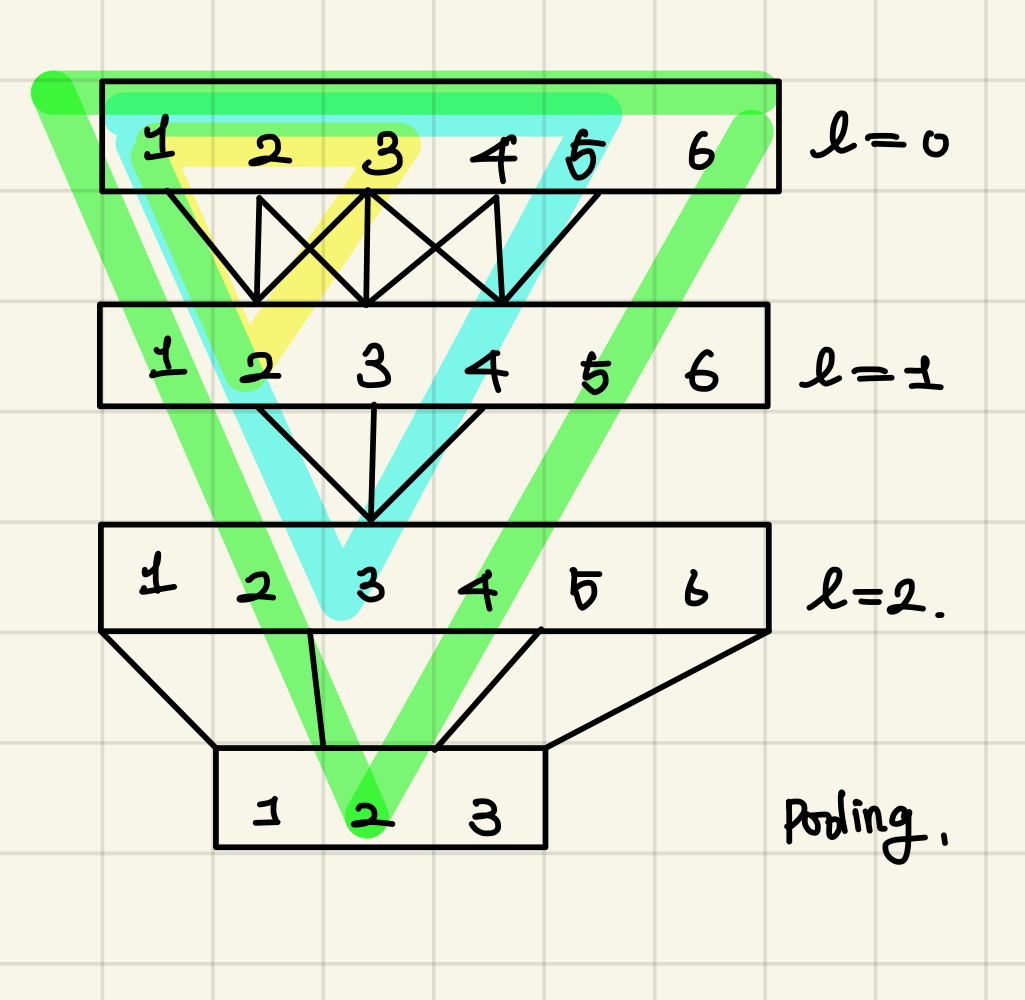
\includegraphics[scale = 0.2]{./fig/image.png}
    \end{center}
    \caption{Simple 1D convolution example whose kernel size is 3 that shows the receptive field with fluorescent colors. After applying two convolutions, the last output is describing the pooling process with kernel size 2, striding 2.}
    \label{fig1}
\end{figure}
As the green triangle in figure \ref{fig1} depicts, the max-pooling with striding 2 increases the receptive field of each node by 1. This implies that $y_2[k,i,j]$ depends on $X[0:2,2i-2:2i+4,2j-2:2j+4]$.
Please note that factor 2 in front of $i,j$ results from the layer after the pooling which is downsamled by factor of 2. Also, note that factoring does not affect to the size of receptive field(it is still 6).
Taking this process into account, the dependence of $y_3$ is trivial, except the fact that the increment of receptive field's size is $2(k-1)$, rather than $k-1$. This is because maxpooling operation downsized the successive layer by half with respect to the original image. 
Thus, the size of receptive field of $y_3[k,i,j]$ is 6 + 4 + 4 + 2 = 16. Again, considering the target index is doubled with respect to input image after passing through the maxpool layers, $y_2[k,i,j]$ depends on $X[0:2,4i-6:4i+10,4j-6:4j+10]$.

\section*{5}
I used following two formulae to solve this problem. Please note that I calculated FLOPS(Floating Point Operations) not MACs(Multy-ACCumulated).
$k$ denotes the filter size with padding $p$ and striding $s$. Also, I denotes the input has $C_{in} \times H_{in} \times W_{in}$, which corresponds to channel, height, and width, respectively.
\begin{align}
    &\text{the number of trainable parameters} = k^2C_{in}C_{out} + C_{out}\\
    &\text{the number of FLOPs} = 2(C_{in} k^2)(C_{out}H_{out}W_{out})\\ 
    &\text{the number of Activation Function Evaluation} = C_{out}\times H_{out} \times W_{out}\\
    &\text{ where } H_{out} = \frac{H_{in} - k + 2p}{s} + 1,\; W_{out} = \frac{W_{in} - k + 2p}{s} + 1
\end{align}
The derivation of the both equation above is as follows.
The number of trainable parameters is summation of one in the kernel and in the bias. 
It is obvious that the kernel has $k^2C_{in}C_{out}$ parameters and the bias has $C_{out}$ parameters.
The number of FLOPs can be calculated by multiplying the number of outputs to the number of operations for each output. 
The number of outputs is $C_{out}\times H_{out} \times W_{out}$, while the number of operation for each output is $(C_{in}\times k \times k) + (C_{in}\times k \times k)$.
Note that the number of operation for each output is summation of the number of multiplication($C_{in}\times k\times k$) and the number of the addition($C_{in}\times k\times k$)\footnote{Taking the following example, it is obviouse. Consider the case of doing inner product of two vectors $\mathbf{a,b}\in\mathbb{R}^3$. Then, it returns $a_1b_1 + a_2b+2 + a_3b_3$ and we can realize that inner product need 3 multiplications and 2 additions. Also, considering the bias term, it result in 3 additions and multiplications}.
Finally, the number of activation function evaluation is equal to output size since activation function applyes to the result of each convolution.
According to these formula above, I compared the number of trainable parameters and that of FLOPs.

To clarify the discussion, I named each convolution layer like figure \ref{fig2}. The results of the calculation in this problem are listed on the table \ref{tab1}, and \ref{tab2}.
Also, the figure \ref{fig3} shows the comparison of module 1 and 2. As the figure \ref{fig3} and table \ref{tab1}, \ref{tab2} describes, module 2 is extremely efficient compared to module 1.
The number of trainable parameter, addition, and multiplication of module 2 is about one-third that of module 1. It is obvious that module 2 has more activation function evaluation since it has more convolution layers and more to be activated.
Eventhough module 2 has more activation function evaluation about 2M, it is still efficient since that difference is not important because the difference of FLOPs between module 1 and 2 is about 800M. 
\begin{figure}[!h]
    \begin{center}
        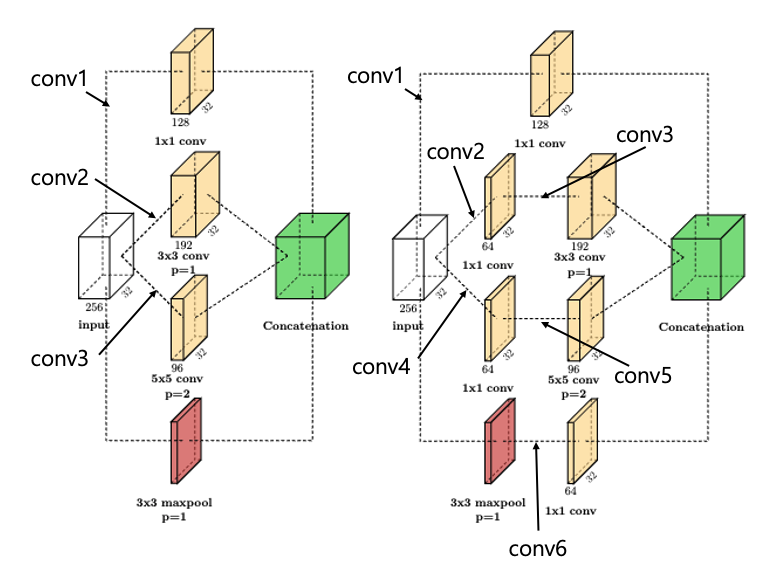
\includegraphics[scale = 0.5]{"./fig/conv.png"}
    \end{center}
    \label{fig2}
    \caption{Name of each convolution layer in this problem}
\end{figure}
\clearpage
\begin{figure}[!h]
    \begin{center}
        \subfigure[]{
            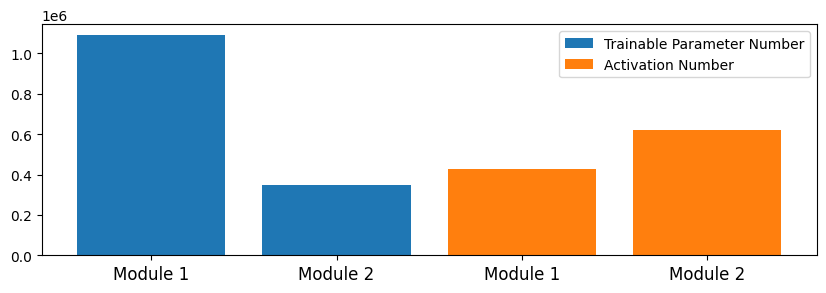
\includegraphics[scale = 0.5]{"./fig/hist1.png"}
        }   
        \subfigure[]{
            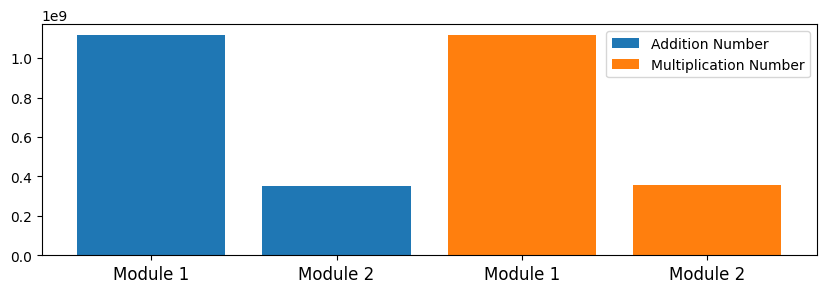
\includegraphics[scale = 0.5]{"./fig/hist2.png"}
        }
    \end{center}
    \caption{The total number of trainable parameters and FLOPs. (a) The number of trainable parameters and activation function evaluation. (b) The number of addition and multiplication}
    \label{fig3}
\end{figure}

\begin{table}[!h]
    \begin{center}
        \begin{tabular}{lllll}
            & conv1    & conv2     & conv3     & TOTAL      \\
            \hline \hline
        trainable paramter & 32,896    & 442,560    & 614,496    & 1,089,952    \\
        addition           & 33,554,432 & 452,984,832 & 629,145,600 & 1,115,684,864 \\
        multiplication     & 33,554,432 & 452,984,832 & 629,145,600 & 1,115,684,864 \\
        activation         & 131,072   & 196,608    & 98,304     & 425,984    
        \end{tabular}
    \end{center}
    \caption{The number of trainable parameters and that of FLOPs in module 1.}
    \label{tab1}
\end{table}

\begin{table}[!h]
    \begin{center}
        \begin{tabular}{llllllll}
                    & conv1    & conv2    & conv3     & conv4    & conv5     & conv6    & TOTAL     \\
                    \hline \hline
        trainable parameter & 32,896    & 16,448    & 110,784    & 16,448    & 153,696    & 16,448    & 346,720    \\
        addition            & 33,554,432 & 16,777,216 & 113,246,208 & 16,777,216 & 157,286,400 & 16,777,216 & 354,418,688 \\
        multiplication      & 33,554,432 & 16,777,216 & 113,246,208 & 16,777,216 & 157,286,400 & 16,777,216 & 354,418,688 \\
        activation          & 131,072   & 65,536    & 196,608    & 65,536    & 98,304     & 65,536    & 622,592   
        \end{tabular}
    \end{center}
    \caption{The number of trainable parameters and that of FLOPs in module 2.}
    \label{tab2}
\end{table}
\section*{6}
In this problem, I tried to reproduce the result of the original paper with AlexNet and MNIST dataset.
I put the code I used in this experiment in the appendix. Here is the design of this experiment. 
To see how to model changes with respect to the portion of noised labels, I repeat the experiment with several randomly noised label ratio. 
\textbf{create\_randomized\_dataset()} function make the randomly labeled dataset given the ratio. The results of this experiment are as follows.(See figure \ref{fig4})
\begin{figure}[!h]
    \begin{center}
        \subfigure[]{
            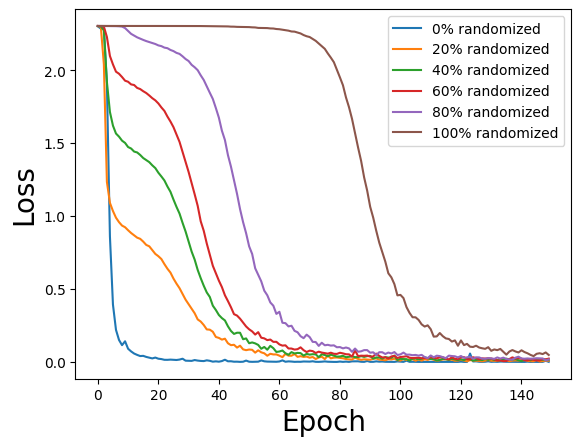
\includegraphics[scale = 0.5]{./fig/fig5.png}
        }
        \subfigure[]{
            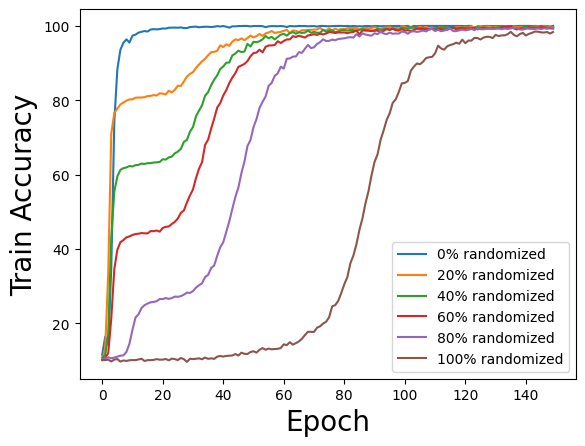
\includegraphics[scale = 0.5]{./fig/fig4.png}
        }
        \subfigure[]{
            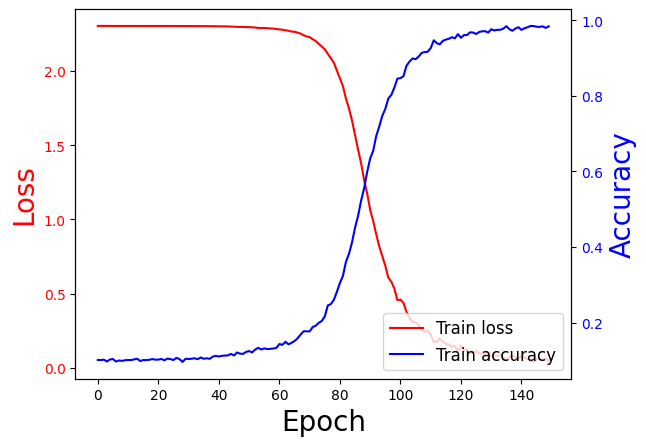
\includegraphics[scale = 0.5]{./fig/fig6.png}
        }
        \subfigure[]{
            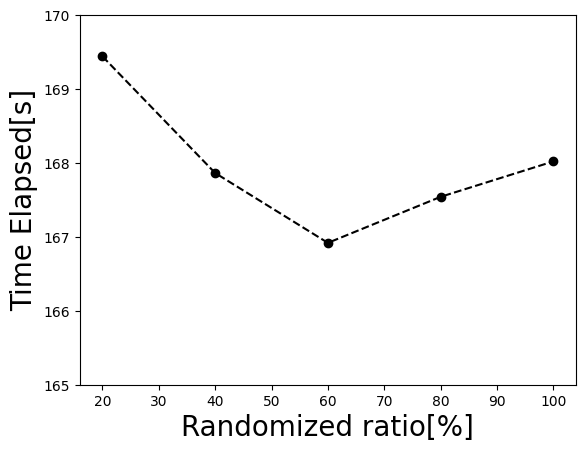
\includegraphics[scale = 0.5]{./fig/fig7.png}
        }
        \subfigure[]{
            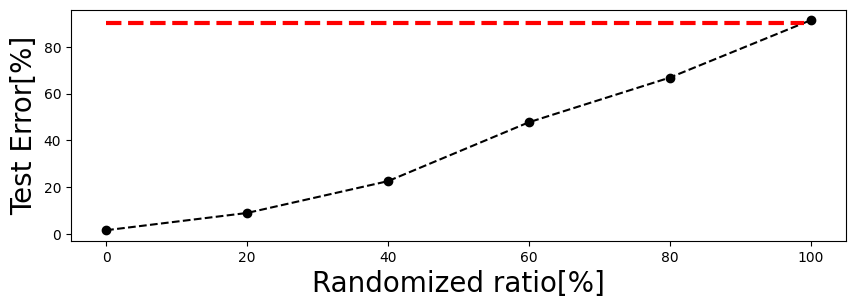
\includegraphics[scale = 0.7]{./fig/fig8.png}
        }
    \end{center}
    \caption{The result of the experiment. (a),(b) The training losses decrease, while the train accuracies increase despite the different ratio of noise. (c) The loss and accuracy curve in training period with 100\% randomized label. (d) The time spent while training doesn't monotonically increase as the randomly noised data becomes majority. (e) The test error converge to 90\% as the randomized label increases.}
    \label{fig4}
\end{figure}
Evnethough the labeled are totally randomized, which implies there is no semantical relation between input and label, the model successfully classify the MNIST dataset in training period.
Eventhough the training losses converge to zero, the test losses are increasing as the randomized ratio of train data increases.
This shows that the model is memorizing the train data when the training. This suggests that the model has sufficient capacity to memorize the whole training data.



\clearpage
\appendix
\section{}
\begin{python}
    import torch
    import torch.nn as nn
    import time
    from torchvision import datasets, transforms
    
    # Make sure to use only 10% of the available MNIST data.
    # Otherwise, experiment will take quite long (around 90 minutes).
    import numpy as np
    
    # Set random seed for reproducibility
    torch.manual_seed(42)
    np.random.seed(42)
    
    learning_rate = 0.1
    batch_size = 64
    epochs = 150
    
    def create_randomized_dataset(train_data, label_ratio):
        subset_indices = np.random.choice(len(train_data), len(train_data)//10, replace=False)
        num_random_labels = int(len(train_data) * label_ratio)
        random_labels = torch.randint(low=0, high=10, size=(num_random_labels,))
        labels = torch.cat((train_data.targets[:num_random_labels], random_labels), dim=0)
        subset = torch.utils.data.Subset(train_data, subset_indices)
        subset.targets = labels
        return subset
    
    # Evaluate the accuracy of the model on the test dataset
    def test_model(model, test_loader):
        model.eval()
        correct = 0
        total = 0
        with torch.no_grad():
            for images, labels in test_loader:
                images, labels = images.to(device), labels.to(device)
                outputs = model(images)
                _, predicted = torch.max(outputs.data, 1)
                total += labels.size(0)
                correct += (predicted == labels).sum().item()
        accuracy = correct / total * 100
        return accuracy
    
    # (Modified version of AlexNet)
    class AlexNet(nn.Module):
        def __init__(self, num_class=10):
            super(AlexNet, self).__init__()
    
            self.conv_layer1 = nn.Sequential(
                nn.Conv2d(1, 96, kernel_size=4),
                nn.ReLU(inplace=True),
                nn.Conv2d(96, 96, kernel_size=3),
                nn.ReLU(inplace=True)
            )
            self.conv_layer2 = nn.Sequential(
                nn.Conv2d(96, 256, kernel_size=5, padding=2),
                nn.ReLU(inplace=True),
                nn.MaxPool2d(kernel_size=3, stride=2)
            )
            self.conv_layer3 = nn.Sequential(
                nn.Conv2d(256, 384, kernel_size=3, padding=1),
                nn.ReLU(inplace=True),
                nn.Conv2d(384, 384, kernel_size=3, padding=1),
                nn.ReLU(inplace=True),
                nn.Conv2d(384, 256, kernel_size=3, padding=1),
                nn.ReLU(inplace=True),
                nn.MaxPool2d(kernel_size=3, stride=2)
            )
    
            self.fc_layer1 = nn.Sequential(
                nn.Dropout(),
                nn.Linear(6400, 800),
                nn.ReLU(inplace=True),
                nn.Linear(800, 10)
            )
    
        def forward(self, x):
            output = self.conv_layer1(x)
            output = self.conv_layer2(output)
            output = self.conv_layer3(output)
            output = torch.flatten(output, 1)
            output = self.fc_layer1(output)
            return output
    
    # Load the MNIST dataset
    train_data = datasets.MNIST(root='./', train=True, download=True, transform=transforms.ToTensor())
    
    # Define the ratios of randomized labels to experiment with
    label_ratios = [0, 0.2, 0.4, 0.6, 0.8, 1.0]
    
    test_data = datasets.MNIST(root='./', train=False, download=True, transform=transforms.ToTensor())
    
    # Define a data loader for the test dataset
    test_loader = torch.utils.data.DataLoader(dataset=test_data, batch_size=batch_size, shuffle=False)
    
    
    device = torch.device("cuda" if torch.cuda.is_available() else "cpu")
    model = AlexNet().to(device)
    loss_function = torch.nn.CrossEntropyLoss()
    optimizer = torch.optim.SGD(model.parameters(), lr=learning_rate)
    losses = []
    times = []
    acc = []
    
    for label_ratio in label_ratios:
        print(f"\nExperiment with {int(label_ratio * 100)}% randomized labels")
        tmp_losses = []
    
        # Create a dataset subset with the specified label ratio
        train_subset = create_randomized_dataset(train_data, label_ratio)
    
        # Define a data loader for the subset
        batch_size = 64
        train_loader = torch.utils.data.DataLoader(dataset=train_subset, batch_size=batch_size, shuffle=True)
    
        # Define the model, optimizer, and loss function
        model = AlexNet().to(device)
        loss_function = torch.nn.CrossEntropyLoss()
        optimizer = torch.optim.SGD(model.parameters(), lr=learning_rate)
    
        # Train the model
        tick = time.time()
        for epoch in range(epochs):
            tmp2_losses = []
            for images, labels in train_loader:
                images, labels = images.to(device), labels.to(device)
    
                optimizer.zero_grad()
                loss = loss_function(model(images), labels)
                tmp2_losses.append(loss.item())
                loss.backward()
                optimizer.step()
            tmp_losses.append(np.mean(tmp2_losses))
        tock = time.time()
        accuracy = test_model(model, test_loader)
        
        # logging
        losses.append(tmp_losses)
        times.append(tock-tick)
        acc.append(accuracy)
        
        print(f"Total training time: {tock - tick}")
    
    \end{python}


\end{document}